\documentclass[12pt, a4paper]{article}
\usepackage{amssymb, amsmath, amsthm}
\usepackage{multirow}
\usepackage{color}
\usepackage[sort&compress]{natbib}
\usepackage{hyperref}
\usepackage{graphicx}
\usepackage{setspace}
\hypersetup{
    pdftitle={Towards a standardized evaluation of multiple imputation routines}
    pdfauthor={Gerko Vink and Andrew Gelman},
    pdfsubject={Evaluating imputation routines},
    pdfkeywords={Multiple imputation, evaluation, simulation, finite population},
    bookmarksnumbered=true,     
    bookmarksopen=true,         
    bookmarksopenlevel=1,       
    colorlinks=false,
    citecolor=blue,
    linkcolor=blue,
    urlcolor=blue,                 
    pdfstartview=Fit,           
    pdfpagemode=UseOutlines,      
    pdfpagelayout=TwoPageRight
}

\singlespacing

\begin{document}
\title{Towards a standardized evaluation of multiple imputation routines}

\author{Gerko Vink}
%\author{Gerko Vink$^{1}$\thanks{Correspondence to: Gerko Vink, Department of Methodology and Statistics, Utrecht University, PO Box 80140, 3508 TC Utrecht, the Netherlands. E-mail: \texttt{G.Vink@uu.nl}}\; and Andrew Gelman$^{2}$\\
%\newline\\
%\small{\textsl{$^1$Department of Methodology and Statistics, Utrecht University}\protect}\\
%\small{\textsl{$^2$Department of Statistics, Columbia University}\protect}\\
%\newline}
\date{}
\maketitle

%%%%%%%%%%%%%%%%%%%%%%%%%%
%% ABSTRACT
%%%%%%%%%%%%%%%%%%%%%%%%%%
\begin{abstract}
Developing new imputation methodology has become a very active field. Unfortunately, there is no consensus on how to perform simulation studies to evaluate the properties of imputation methods. In this paper I propose a move towards a standardized evaluation of imputation methods. To demonstrate the need for standardization, I highlight a set of potential pitfalls that bring forth a chain of potential problems in the objective assessment of the performance of imputation routines. This may lead to suboptimal use of multiple imputation in practice. Additionally, I suggest a course of action for simulating and evaluating missing data problems. 
\end{abstract}

%%%%%%%%%%%%%%%%%%%%%%%%%%
%% INTRODUCTION
%%%%%%%%%%%%%%%%%%%%%%%%%%
\section*{Introduction}
\label{intro}

Multiple imputation \citep{rubin1987} is a state-of-the-art technique for drawing valid conclusions from incomplete data, and is increasingly used in many substantive fields, such as medicine \citep[see e.g.][]{pulkki2015cumulative,alkire2015global,stinesen2015reduced}, psychology \citep[e.g.][]{sorbi2014medium}, economics \citep[e.g.][]{wong2015economic,dafoe2013democratic,allan2015determinants}, sociology \citep[e.g.][]{crowley2014flexible,de2014religiosity} and official statistics \citep[e.g.][]{little2012calibrated,klausch2015selection}. 

The technique has earned a permanent spot in research and policy making, demonstrated e.g. by the detailed manual created by the National Research Council \citep*{little2012prevention}. Although a top-down enforcement of valid ways to handle missing data is not yet very pronounced, an increasing amount of researchers are embracing multiple imputation techniques. After all, the principle of multiple imputation is very intuitive.

The idea behind multiple imputation is to impute (fill in) the missing values multiple times to obtain a valid estimate of what could have been. The multiple datasets that are thus obtained can be analyzed by standard techniques and the analysis results can be combined into a single inference. In contrast to ad hoc methods for dealing with missing values (e.g. listwise deletion, mean imputation, regression imputation, last observation carried forward), multiple imputation properly takes the sources of uncertainty that are related to the missingness problem into account.

The quality of a solution obtained by multiple imputation depends on the statistical properties of the incomplete data and the degree to which an imputation procedure is able to capture these properties when modeling missing values. In general it holds that modeling missing data becomes more challenging when the amount of missingness increases. However, when (strong) relations in the data are present, the observed parts can hold great predictive power for the models that estimate the missingness. In that case, multiple imputation would be substantially more efficient than the ubiquitous listwise deletion.

When evaluating the statistical properties (and thereby the practical applicability) of new imputation methodology, researchers most often make use of simulation studies. In such studies a complete data set is usually generated from a statistical model, another model is used to induce missingness, and a set of evaluation criteria is postulated to evaluate the performance of the imputation method. However, no golden standard has been established and, as a result, validity of the simulation and evaluation procedures may differ tremendously from one developer to another. 

The purpose of this paper is threefold: First, I raise some concerns with respect to evaluating imputation methodology. These concerns stem from careful consideration with fellow `imputers' and from encounters as a reviewer for statistical journals. Second, I provide imputation methodologists with a suggested course of action when simulating missing data problems. This suggested approach should identify a common ground, but is in no way intended as an absolute solution. This identifies the third purpose of this paper: discussion. I hope to elicit critical thinking with respect to the problems at hand. We are all convinced that our methodology has some merit. But for sake of progress it would be much more advantageous if the aim of our evaluations would go beyond \emph{proving the point} and would legitimately consider the statistical properties. 

%%%%%%%%%%%%%%%%%%%%%%%%%%
%% INTRODUCTION
%%%%%%%%%%%%%%%%%%%%%%%%%%
\section*{Why some evaluations should not be trusted}
As of today, there is no consensus on how to perform simulation studies to evaluate the properties of imputation methods. Typically, the developer of a new imputation routine does some tests by simulations, but these tests differ across developers. This brings forth a chain of potential problems in the objective assessment of the performance of imputation routines that may lead to suboptimal use of multiple imputation in practice. To demonstrate the broad impact of these problems, I subdivide the problems in the following three distinct categories: problems with data generation, problems with missingness generation and problems with performance evaluation. I further detail the impact these problems may have on the validity of the performance evaluation of the imputation routines. 

\subsection*{Data generation problems}
To evaluate the ability of an imputation routine to handle the nonresponse model, a form of truth has to be established. Those who perform simulation studies are in the luxury position to establish the truth beforehand, either by generating data from a statistical model, or by sampling data from a sufficiently large observed set. However, when generating data, two easily overlooked problems may arise.  

First, data are often generated following the model (or distribution) that is also used for imputing the data. The performance of the imputation approach is then deemed good, which is no surprise as the evaluated conditions are in favor of the problem that is studied. Although such procedures may be statistically relevant, the approach would be no good for even the simplest case. Such simulations pose serious threats to the applicability of the method as real-life data hardly ever follow a given theoretical distribution. 

Second, data are often generated such that the problem that is being studied is most pronounced. This results in simulated data that contains very valuable information structures, i.e. the correlations between groups of variables may be very pronounced. In other words, no matter what type of missingness is induced, the observed parts of the data may still hold much, if not all, of the information about the missing part and the performance of the imputation procedure is not surprisingly evaluated as very good. Also, it may be that the relations in real-life data are rarely as pronounced as the problem that is being studied.

\subsection*{Missingness generation problems}
In order to obtain valid imputation inference, the imputation model must capture the essence of the true nonresponse mechanism \citep{meng1994multiple}. The model - if any - that is used to generate the missingness is usually assumed to be random (MAR) or completely random (MCAR). Missingness mechanisms that are not random (MNAR) and mechanisms that are considered non-ignorable \citep[see e.g.][]{rubin1976inference}, are generally ignored during evaluation of imputation methodologies, except for those methods that are specifically targeted at non-ignorable applications.

With MCAR missingness mechanisms, the probability to be missing is the same for all cases. This is a necessary simulation condition for evaluating the performance of imputation procedures. If an imputation method is not able to solve the problem (i.e. yield valid inference) under MCAR, the statistical properties of the procedure are not sound. Sadly, the straightforward case of MCAR is often neglected from simulation studies and focus is drawn to the evaluation of MAR mechanisms only. Alternatively, some studies limit their evaluations to MCAR mechanisms only, which in my view may be far too simplistic. 
\begin{figure}[t!]
  \resizebox{\textwidth}{!}{
    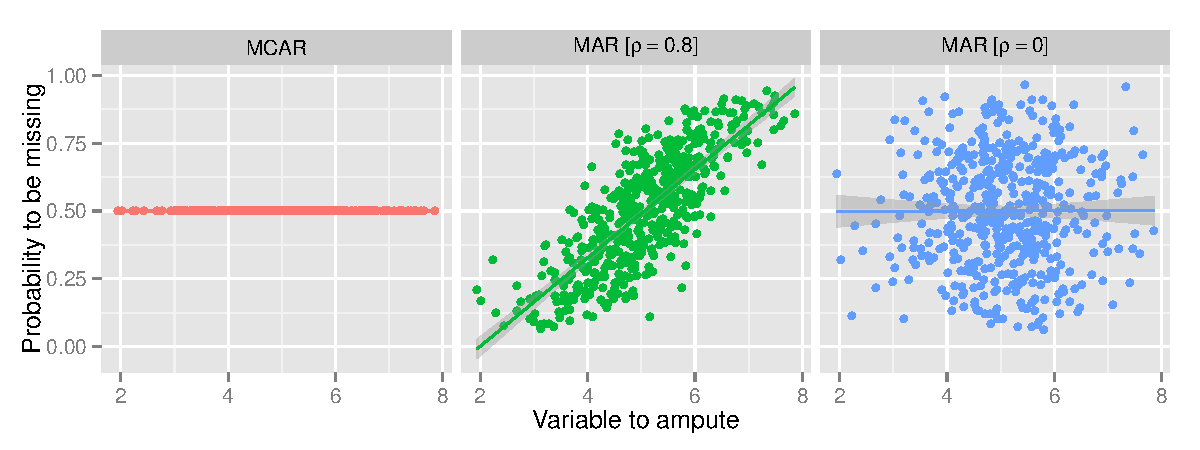
\includegraphics[scale=1]{figures/plot_mmech.pdf}
  }%
  \caption{Three missingness mechanisms that yield approximately 50 percent missingness ($N=500$). Displayed are a MCAR mechanism, a right-tailed MAR mechanism generated from bivariate normal data with correlation $\rho=.8$ and the same MAR mechanism, now generated from bivariate normal data with correlation $\rho= 0$.}
  \label{fig:mis.mech}
\end{figure}

With MAR missingness mechanisms, the probability to be missing is the same within groups of cases defined by the observed data only (e.g. males are less likely to disclose their weight, but gender is observed). The essence here is that the observed relations in the data are used to induce missingness during simulation (e.g. weight is made incomplete based on gender), but these relations may be weak, or non-existent. 

When MAR is induced based on weaker relations in the data, claims for a method's applicability to situations where the missingness is random become less valid. When MAR is induced from data without multivariate relations, the inferential implication of the missingness would mimic those of MCAR. This problem is generally overlooked in simulation studies and the procedure to generate missing data is often insufficiently described in resulting publications. Figure \ref{fig:mis.mech} demonstrates two realizations of missingness mechanisms under MAR mechanisms derived from data with different multivariate relations. 

It is obvious that the MAR missingness generated from data with low correlation would yield similar inference to the MCAR missingness, even though the missingness is clearly random. The simulation results from Table 1 confirm this. A detailed simulation setup can be found in Appendix A. 

As expected, under genuine MAR missingness, i.e. the missingness probabilities differ conditional on the level of the incomplete variable, the performance of complete case analyses drops dramatically. For \emph{spurious} MAR, i.e. the conditional probabilities remain the same over the level of the incomplete variable, the performance is comparable to that under MCAR. In fact, this would amount to one of the special cases under which complete case analysis would be more efficient than multiple imputation \citep[see e.g.][p. 48]{fimd}: the missingness does not depend on the incomplete variable. This property might be useful in practice, but considering it as a condition to evaluate performance under MAR missingness is useless. 

Although one cannot definitively verify if the missingness is random - after all, for every MNAR mechanism there is a MAR mechanism with equal fit \citep{molenberghs2008every} - it can be argued that MNAR is the more likely mechanism for real life missingness scenarios. In such cases, an indication of the validity of the obtained inference, given that the assumed missingness mechanism is suspected to be invalid, may be obtained by performing sensitivity analysis \citep[see e.g.][part 5]{molenberghs2014handbook}.

% latex table generated in R 3.2.2 by xtable 1.8-0 package
% Thu Feb  4 16:27:54 2016
\begin{table}[t]
\caption{Inferences obtained by complete case analysis (CCA) and multiple imputation over 1000 simulations. Displayed are the bias, coverage rate (cov) of the 95\% confidence interval and the confidence interval width (ciw). Imputations are generated by Bayesian linear regression imputation.}
\centering
\begin{tabular}{rlccccccc}
  \hline
 	& &\multicolumn{3}{c}{CCA} &&\multicolumn{3}{c}{imputation}	\\\cline{3-5}\cline{7-9}
 \multicolumn{2}{c}{mechanism}	& bias & cov & ciw && bias & cov & ciw \\ 
  \hline
  $[\rho = .8]$ &mcar & 0.001 & 0.959 & 0.179 && -0.001 & 0.946 & 0.156 \\ 
  $[\rho = .8]$ &mar & {\color{red} 0.334} & {\color{red} 0.000} & 0.169 && 0.004 & 0.955 & 0.195 \\ 
  $[\rho = .0]$ &mar & 0.003 & 0.973 &{\color{red} 0.180} && 0.013 & 0.947 & 0.311 \\    \hline
\end{tabular}
\label{tab:mis.mech}
\end{table}  

The amount of missingness that is used to simulate the performance of imputation methods differs between studies. Some studies use only 10\% missing data where other studies push the limits to additionally investigate the performance under at least 50\% missing data. This inconsistent display of simulation results may impact the objectivity of meta-evaluations over imputation methods, as one method's performance may appear to be favorable because of the less stringent simulation conditions. This ultimately may lead to statisticians recommending a less efficient method to applied researchers, thereby limiting the efficiency of the imputation approach and unnecessarily lowering the statistical power.

\subsection*{Performance evaluation}
The evaluation criteria used to assess imputation performance vary from one developer to another. This is not surprising as people from different fields could have a different focus on the problem at hand. However, because multiple imputation was designed as a mode for statistical inference, a minimal set of statistical properties should at least be evaluated. I highlight four aspects of evaluation that should be considered when evaluation imputation routines. 

First, developers often only inquire about the `accuracy' (i.e. how well can the method reproduce the original data). The goal of multiple imputation is not to reproduce the data, but to allow for obtaining valid inference given that the data are incomplete. We are interested in the correct answer to the research question; not in the truth itself. This means that, given the framework provided by \citep{rubin1987}, statistical properties such as bias, confidence intervals and the coverage rate of the confidence intervals should be studied. After all, the 95\% confidence interval should contain the `true' value at least 95 out of 100 times \citep[][p. 591]{neyman1934two}.

Second, the performance of imputation procedures on distributional properties is often ignored in simulation studies, and even though the estimates on the analysis level may be justified, some methods can yield imputations that may seem completely invalid to applied researchers. For example, one could very accurately estimate average human height by filling in negative values and values that are unrealistically large. While the obtained inference could still be valid under such imputations, the plausibility of the imputed values given the observed data should be under scrutiny. Rather, one would prefer an imputation technique to yield both valid inference and plausible imputations. It should be studied if an imputation method is prone to deliver such impractical results, and if so, under what conditions.

Third, sampling variation has always been an essential part of the evaluation of multiple imputation methodology. However, in order to obtain information about a method's ability to handle the missing data problem, or to objectively compare methods on their ability to correct for missingness, it is not necessary to take sampling variation into account \citep{vink2014pooling}. After all, we are interested only in the missing data mechanism, and are not considering the noise induced by the sampling mechanism for evaluation in such studies.

Last, when the evaluator is on the verge of drawing conclusions about the performance of the imputation routine, the performance should be carefully qualified. Comparing the performance of an imputation routine given a population (or true) parameter allows for quantitative evaluation. However, in order to pose qualitative statements about the performance on simulated conditions, comparative methodology is required. For example, when claiming that imputation performance is unacceptable when deviations from normality become rather stringent, such performance is highly dependent on the simulation conditions that are used. For a well-balanced judgement about the severity of the performance drop, comparative simulations with e.g. nonparametric models should be executed. A method may perform badly, but if it still outperforms every other approach, it may yet be of great practical relevance.


\section*{Suggested course of action}
\subsection*{Step 1. Obtain truth}
The evaluator must to decide whether there is a need for sampling variance in the simulations scheme. If sampling variance cannot be omitted from the simulation scheme, two approaches are possible:
\begin{enumerate}
  \item Model-based simulation: draw samples from a known probability distribution, such as the multivariate normal distribution. The theoretical parameters under which the samples are obtained will serve as the comparative truth during the simulations. 
  \item Design-based simulation: sample data from a sufficiently large set. The parameters of the sufficiently large set will serve as the comparative truth during the simulations. This approach is often used in situations where a probability distribution is not available, or where real-life data structures are of interest. Applications of design-based simulation are often found in official statistics. A benefit of design-based simulation is the ability to use real-life observed data structures. 
\end{enumerate}
For situations where sampling variance is not of interest, the sampling process can be omitted and a single complete dataset can simply be obtained by model- or design-based approaches. The parameters of that single complete set will serve as comparative truth. This process is computationally convenient, because only a single complete datasets has to be considered during all of the simulations. One needs to realize, however, that the conventional pooling rules \citep[cf.][p. 76-77]{rubin1987} do not apply for finite population inference and that alternative pooling rules need to be used \citep{raghunathan2003multiple,vink2014pooling}. 

\subsection*{Step 2. Induce missingness}
First, one should always consider MCAR missingness, i.e. the scenario where the missing values are missing at random and the observed values are observed at random. Under MCAR, the statistical properties of the observed data given the missing data are known and any imputation routine that cannot at least mimic the performance of the observed data inference, should be deemed inefficient in the scope of the simulation.  

Next, missing data should be induced conform a model that is dependent on the observed data. A straightforward technique for inducing different forms of univariate MAR missingness is described in \citet[][p. 63; see Figure \ref{fig:mar}]{fimd} and a generalization to multivariate MAR missingness can be found in \citet[][Appendix B]{van2006fully} and \citet[][\S 5.2.3]{brand1999development}. If the missingness is to be induced in longitudinal data, autoregressive MAR models \citep[e.g. cf.][model 2 and model 3]{shara2015randomly} can be useful. 

\begin{figure}[t!]
\begin{center}
  \resizebox{\textwidth}{!}{
    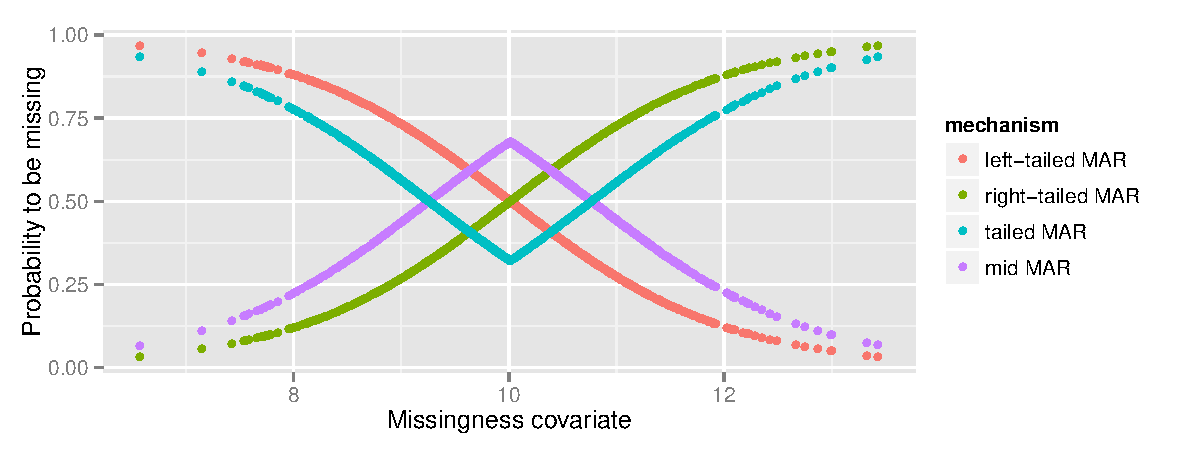
\includegraphics[scale=1]{figures/plot_mar.pdf}
  }%
  \caption{Examples of four random missingness mechanisms that yield approximately 50 percent missingness. For negatively correlated missingness covariates the resulting mechanisms are reversed. }
  \label{fig:mar}
  \end{center}
\end{figure}
Third, it is advisable to investigate varying shapes of MAR missingness to achieve a more realistic indication of the robustness of the imputation performance across the range of random missingness. Given the simulated data-distributions, one random missingness model may be far more disastrous to the observed information than another model. This may influence the performance of some (but not necessarily all) imputation routines For example, inference from  hot-deck techniques such as predictive mean matching \citep{little1988missing, rubin1986statistical} may be more severely impacted by large amounts of one-tailed missingness than inference from parametric techniques. It would be a shame to overlook such results due to the focus on a single MAR mechanism. 

Fourth, the amount of missingness must be varied. Remember that missingness is only ignorable under MAR when the parameter of the data is distinct and a-priori independent from the parameter of the missing data process. Under MAR missingness we assume that we may use the observed data to make inferences about the joint (observed and unobserved) data. 

The dependency of the procedure on the assumption under which we obtain inference is only influenced by the amount of missingness. If there is no missingness - or if there is no data, for that matter - the inference does not depend on the assumption. Alternatively, the validity of assumptions become increasingly important when the missingness increases. Since we control the MAR mechanism, the assumption under which we may solve the missing data problem should hold and it is only fair to assess performance under stringent missingness conditions. I therefor propose, for all mechanisms, to evaluate at least the following univariate missingness percentages when evaluating imputation routines:

\begin{itemize}
  \item 10\% missingness: Depending on the size of the data, this percentage can be considered as a lower bound of realistic evaluation. Anything less than 10\% may be of little influence on the true data inference. Performance of a missing data method should at least be acceptable for most missing data problems. 
  \item 25\% missingness: This is a fair amount of missingness and will, depending on the observed data information, have a noticeable influence on the completed data inference. When compared to the condition with 10\% missingness, the inference obtained under 25\% missingness should be less certain (i.e. confidence/credibility interval width should increase), but estimates should still be properly covered and the statistical properties of the missing data method should be sound. In practice, at least to my experience in social sciences and official statistics, 25\% univariate missingness can easily be considered as a realistic missingness percentage. 
  \item 50\% missingness: Performance under 50\% percent simulated missingness will most likely be impacted severely. Depending on how the missingness mechanism interacts with the simulated data, some imputation techniques may yield estimates that are undercovered such that the completed data inference should not be deemed valid anymore. If a method yields acceptable inference under 50\% MAR missingness, we can determine that the statistical properties of the imputation methodology are sound. 
\end{itemize}
Although I limit the focus here to ignorable nonresponse, the above suggested proportions are equally applicable to simulations under non-ignorable nonresponse.

Fifth, the used missingness mechanism should be detailed, either graphically or written as a function of the data. Often, when inducing missingness, authors remain vague about the actual missingness mechanism under investigation and, even worse, some authors only report something like
\begin{quote}
\emph{We generated missing data following a MAR missingness mechanism.}
\end{quote}
This should be considered unacceptable as claims about the validity of the multiple imputation inference depends heavily on the simulated missingness mechanism. 

\subsection*{Step 3. Evaluate performance}
It is wise to evaluate the performance of complete case analysis (aka listwise deletion) in all simulated conditions. We know the theoretical properties of complete case analysis, which makes the technique useful as a point of departure when evaluating multiple imputation performance. 
The evaluation criteria may depend on the estimand. When descriptive statistics are the goal and when statistical inference would not be of interest, bias of the estimates would still apply, but standard errors are generally ignored. Chances are that for those who focus on descriptive statistical applications, multiple imputation would not be the mode of choice. In general, I would say that each multiple imputation routine should be evaluated on at least the following points:
\begin{itemize}
  \item \emph{Bias:} Results should preferable be unbiased. However, the way bias is considered can greatly influence the interpretation of the results. For example, a negligible absolute bias for a parameter for which the true value is zero, would yield infinite bias when relative bias is considered. The way bias is computed should therefore be carefully chosen and described. 
  \item \emph{Interval width:} The way the confidence interval is calculated should be described. Wider intervals are associated with more uncertainty and the more narrow interval that is still properly covered indicates a sharper inference. However, inference from a wider interval that is properly covered is to be considered more valid when compared to a more narrow interval that is not properly covered anymore. 
  \item \emph{Coverage:} Coverage of a 95\% interval should in theory be $\geq 95$, where a coverage of 95\% would be most efficient. Undercoverage (when estimation is too liberal) may be an indication of invalid inference, while overcoverage (when estimation is too conservative) tells us that efficiency could still be gained. 
  \item \emph{Distributional characteristics:} In practice, the distribution of the incomplete data may differ greatly from the observed data. Under anything but the MCAR assumption, this can be expected. When evaluating imputations, the distributional shapes should be checked and diagnostic evaluations should be performed \citep[see][for an detailed overview of diagnostic evaluation for multivariate imputations]{abayomi2008diagnostics}. When anomalies are found, and if the imputation method is valid, there should be an explanation, especially in the controlled environment of a properly executed simulation study. 
  \item \emph{Plausibility of the imputed values:} Plausible imputations - imputations that could be real values if they had been observed - are not a necessary condition for obtaining valid inference. However, in practice, especially when the imputer and the analyst are different persons, plausibility of imputations may be a desired property. When evaluating imputation routines, the evaluator should mention whether the routine is prone to deliver implausible values. 
  \item \emph{Convergence of the algorithm:} Most contemporary imputation techniques rely on iterative algorithms, such as the Gibbs sampler, where some algorithms are critically considered to be possibly incompatible Gibbs samplers \citep[PIGS,][]{li2012imputing}. The convergence of all iterative algorithms should always be considered and if non-convergence is suspected, the inference resulting from the imputations should not be considered.  
  \end{itemize}
For evaluations of model-based simulations, it could be convincing to demonstrate a method's applicability to real-world missing data problems. This can, for example, be achieved by obtaining and imputing a fully observed set of variables, wherein the missingness is mimicked from a similar, incomplete set. Alternatively, an incomplete set could be obtained and truth could be established by removing the incomplete cases from the data. However, the real-world missingness would then be omitted.

\section*{Discussion}
This document is aimed at establishing a common ground for the evaluation of imputation routines. Such a common ground would be the basis of a standardized evaluation. This allows for fair and efficient comparisons between imputation techniques. Ultimately, it would be desirable to evaluate every imputation routine against the same standardized set in order to quantify the statistical properties across imputation routines. If properly executed, this would allow for careful matching of imputation methodologies to new missing data problems. 

\section*{Appendix A: Simulation setup}
Let $Y=(Y_{obs},Y_{mis})$ be an incomplete semicontinuous variable, where $Y_{obs}$ and $Y_{mis}$ denote the observed values and the missing values in $Y$, respectively.  Further, $X=(X_1,...,X_k)$ is a set of $k$ fully observed covariates, where $X_{obs}$ and $X_{mis}$ correspond to the observed an missing parts in $Y$ and where $X_j$ would indicate the $j$th variable in $X$, with $j=1,\dots, k$. Finally, let $R$ be a response indicator that is 1 if $Y$ is observed and 0 if $Y$ is missing.

To prove the point, I generated a single data set from the multivariate normal distribution with means
\begin{equation*}\label{meanmatrix}
\mu= \bordermatrix{&	 \cr
 Y	&5	\cr
{ X}_1	&10	\cr
{ X}_2	&10	},
\end{equation*}
and covariance matrix
\begin{equation*}\label{covmatrix}
\Sigma = \bordermatrix{& Y &{ X}_1 &{ X}_2	 \cr
 Y	&1	&0.8	&0\cr
{ X}_1	&0.8	&1	&0\cr
{ X}_2	&0	&0	&1}.
\end{equation*}

Three incomplete sets were then generated, wherein random missingness was imposed in $Y$ in three ways. First, I left the observed data \emph{observed at random} to impose MCAR missingness following the mechanism 
\begin{equation*}
P(R=0|Y_{obs},Y_{mis}, X_j)=P(R=0)=.50.
\end{equation*}
Next, I created random missingness in $Y$ according to the following MAR missingness mechanism
\begin{equation*}
P(R=0|Y_{obs},Y_{mis}, X_j)=P(R=0|Y_{obs}, X_j),
\end{equation*}
by using a random draw from a binomial distribution of the same length as $Y$ and of size 1 with missingness probability equal to the inverse logit
\begin{equation*}
P(R=0)=\frac{e^{a}}{(1+e^{a})}.
\end{equation*}
where $a=(\mu_{X_j}-X_{ij})/\sqrt{\mathbb{E}[X_{ij} - \mu_{X_j}]}$ in order to create approximately 50\% right-tailed MAR missingness. I followed this procedure twice; once for each $X_j$. 

The three resulting incomplete data sets were then imputed with package \texttt{mice} \citep[][v2.25]{mice} in \texttt{R} \citep[][v3.2.3]{R}, with Bayesian linear regression imputation (\texttt{mice.impute.norm}) as the imputation routine.  The completed-data analyses were combined into a single inference following the rules described in \citet{vink2014pooling}. 

\bibliography{bibliography}
\bibliographystyle{apalike}
\end{document}